\documentclass[10pt, a4paper]{exam} 

\usepackage[brazil]{babel}
\usepackage[utf8]{inputenc}
\usepackage{listings}
\usepackage{multicol}
\usepackage{multirow}
\usepackage{caption}
\usepackage{graphicx}
\usepackage{amsmath}
\extraheadheight{2cm}
\extrawidth{2cm}

\begin{document}
	\renewcommand{\solutiontitle}{\noindent\textbf{Solução:}\enspace}
	\qformat{\textbf{Questão \thequestion:}\hfill[\pointsofquestion{\arabic{question}} \points]}
	\hqword{Questões} 			
	\hpgword{Páginas} 			
	%\addpoints
	\bracketedpoints
	\setlength\linefillheight{.6cm} %distância entre linhas
	
%	\pagestyle{headandfoot}
%
%	\lhead[]{}
%	\chead[]{}
%	\rhead[]{}
%	
%	\headrule
%	\footrule
%	\lfoot{}
%	\cfoot{Página \thepage\ de \numpages{}}
%	\rfoot{}
\pagestyle{headandfoot}
\lhead{\bf Universidade Estadual de Campinas - Instituto de Computação (IC/Unicamp)\\Disciplina Aprendizado de Máquina (MO444)\\ Professor: Jacques Wainer\\Atividade 1, \today}
\chead{}
\rhead{\bf Aluno: Luiz Alberto Ferreira Gomes\\ RA:007275}

\lfoot{}
\cfoot{Página \thepage\ de \numpages{}}
\rfoot{}
	
	\vspace{0.1in}
	\printanswers
	
	\begin{questions}	    
	    \question
	    Faça o PCA dos dados (sem a última coluna). Se voce quiser que os dados transformados tenham 80\% da variância original, quantas dimensões do PCA vc precisa manter?
	    \begin{solution}
	    	
			A Tabela 1 apresenta a saída parcial do comando \verb|summary(pca.output)|. A variável \verb|pca.output| é a variável do script em R (ver Anexo I) que armazena o retorno da chamada da função \verb|prcomp| que, por sua vez, calcula o PCA sobre os dados originais. 
			Nessa tabela, a soma acumulada da variância (\textit{Cumulative Proportion}) é maior do que 80\% somente a partir do componente 13 (PCA13). Então, para se atingir a variância pedida no exercício serão necessárias 13 dimensões.
			
			\begin{center}
				\setlength{\tabcolsep}{1.8pt}
				\renewcommand{\arraystretch}{2}
				\scriptsize
				\begin{tabular}{rrrrrrrrrrrrrrrr}
				  \hline
				 & PC1 & PC2 & PC3 & PC4 & PC5 & PC6 & PC7 & PC8 & PC9 & PC10 & PC11 & PC12 & PC13 \\ 
				  \hline
				Standard deviation & 7.1953 & 4.8073 & 3.5561 & 2.9219 & 2.8577 & 2.6019 & 2.3214 & 2.2474 & 1.8183 & 1.6883 & 1.6036 & 1.5417 & 1.4858 \\ 
				  Proportion of Variance & 0.3119 & 0.1392 & 0.0762 & 0.0514 & 0.0492 & 0.0408 & 0.0325 & 0.0304 & 0.0199 & 0.0172 & 0.0155 & 0.0143 & 0.0133 \\ 
				  Cumulative Proportion & 0.3119 & 0.4511 & 0.5273 & 0.5787 & 0.6279 & 0.6687 & 0.7012 & 0.7316 & 0.7515 & 0.7687 & 0.7842 & 0.7985 & 0.8118 \\ 
				   \hline
				\end{tabular}
				\captionof{table}{Saída do comando summary da linguagem R}
			\end{center}
		\end{solution}
	    
	    \question
	    Treine uma regressão logística no conjunto de treino dos dados originais e nos dados transformados. Qual a taxa de acerto no conjunto de teste nas 2 condições (sem e com PCA)? 
	     \begin{solution}
	    	
	  		A taxa de acertos (ou acurácia) pode ser calculada a partir dos dados extraídos das tabelas de confusão, geradas pelo script em R (ver Anexo I), para as duas condições pedidas no exercício:
		   \begin{multicols}{2}
		    \begin{center}
				GLM sem PCA:\vspace{3pt}
				\begin{tabular}{lr|r|r|}
					\cline{3-4}
				 	& & \multicolumn{2}{c|}{Predição} \\
				  	\cline{3-4}
				 	& & 0 & 1 \\ 
				  	\hline
					\multicolumn{1}{ |c| }{\multirow{2}{*}{Real} } & 
					\multicolumn{1}{ |c| }{0} & TN = 115 & FP = 56 \\ \cline{2-4}
				 	\multicolumn{1}{|c|}{} 	&
				 	\multicolumn{1}{|c|}{1} & FN = 44 & TP = 61 \\ \cline{2-4}
				 	\hline
				\end{tabular}
				\captionof{table}{Tabela de confusão.}
			\end{center}
			\begin{equation}
				\begin{split}
					Acuracia & = \frac{TN + TP}{TN+TP+FN+FP}\\
					& = \frac{115 + 61}{115+61+44+56} \\
					& = 0.6376
				\end{split}
			\end{equation}
			\columnbreak
			\begin{center}
				GLM com PCA:\vspace{3pt}
				\begin{tabular}{lr|r|r|}
					\cline{3-4}
				 	& & \multicolumn{2}{c|}{Predição} \\
				  	\cline{3-4}
				 	& & 0 & 1 \\ 
				  	\hline
					\multicolumn{1}{ |c| }{\multirow{2}{*}{Real} } & 
					\multicolumn{1}{ |c| }{0} & TN = 73 & FP = 52 \\ \cline{2-4}
				 	\multicolumn{1}{|c|}{} 	&
				 	\multicolumn{1}{|c|}{1} & FN = 86 & TP = 65 \\ \cline{2-4}
				 	\hline
				\end{tabular}
				\captionof{table}{Tabela de confusão.}
			\end{center}
			\begin{equation}
				\begin{split}
					Acuracia & = \frac{TN + TP}{TN+TP+FN+FP}\\
					& = \frac{73 + 65}{73+65+86+52} \\
					& = 0.5000
				\end{split}
			\end{equation}
			\end{multicols}
			A taxa de acerto do GLM sem pca foi de \textbf{0.6376} (equação 1) e do GLM com pca foi \textbf{0.5000} (equação 2).
	      \end{solution}
	    \pagebreak
	    \question
	    Treine o LDA nos conjuntos de treino com e sem PCA e teste nos respectivos conjuntos de testes. Qual a acurácia nas 2 condições? 
	     \begin{solution}
	    	A taxa de acertos (ou acurácia) pode ser calculada a partir dos dados extraídos das tabelas de confusão, geradas pelo script em R (ver Anexo I), para as duas condições pedidas no exercício:
	    \begin{multicols}{2}
		    \begin{center}
				LDA sem PCA:\vspace{3pt}
				\begin{tabular}{lr|r|r|}
					\cline{3-4}
				 	& & \multicolumn{2}{c|}{Predição} \\
				  	\cline{3-4}
				 	& & 0 & 1 \\ 
				  	\hline
					\multicolumn{1}{ |c| }{\multirow{2}{*}{Real} } & 
					\multicolumn{1}{ |c| }{0} & TN = 127 & FP = 48 \\ \cline{2-4}
				 	\multicolumn{1}{|c|}{} 	&
				 	\multicolumn{1}{|c|}{1} & FN = 32 & TP = 69 \\ \cline{2-4}
				 	\hline
				\end{tabular}
				\captionof{table}{Tabela de confusão.}
			\end{center}
			\begin{equation}
				\begin{split}
					Acuracia & = \frac{TN + TP}{TN+TP+FN+FP}\\
					& = \frac{127 + 69}{127+69+32+48} \\
					& = 0.7101
				\end{split}
			\end{equation}
			\columnbreak
			\begin{center}
				LDA com PCA:\vspace{3pt}
				\begin{tabular}{lr|r|r|}
					\cline{3-4}
				 	& & \multicolumn{2}{c|}{Predição} \\
				  	\cline{3-4}
				 	& & 0 & 1 \\ 
				  	\hline
					\multicolumn{1}{ |c| }{\multirow{2}{*}{Real} } & 
					\multicolumn{1}{ |c| }{0} & TN = 73 & FP = 52 \\ \cline{2-4}
				 	\multicolumn{1}{|c|}{} 	&
				 	\multicolumn{1}{|c|}{1} & FN = 86 & TP = 65 \\ \cline{2-4}
				 	\hline
				\end{tabular}
				\captionof{table}{Tabela de confusão.}
			\end{center}
			\begin{equation}
				\begin{split}
					Acuracia & = \frac{TN + TP}{TN+TP+FN+FP}\\
					& = \frac{73 + 65}{73+65+86+52} \\
					& = 0.5000
				\end{split}
			\end{equation}
			\end{multicols}
			A taxa de acerto do LDA sem pca foi de \textbf{0.7101} (equação 3) e do LDA com pca foi \textbf{0.5000} (equação 4). 
	      \end{solution}

		
	    \question 
	    Qual a melhor combinação de classificador e PCA ou não? 
	    
	     \begin{solution}
	    	A Figura 1, com as acurácias geradas pelo script em R (ver Anexo I), mostra que a melhor combinação de classificadores e PCA - responsável pela maior precisão - foi \textbf{o LDA sem PCA.}
			\begin{center}
  				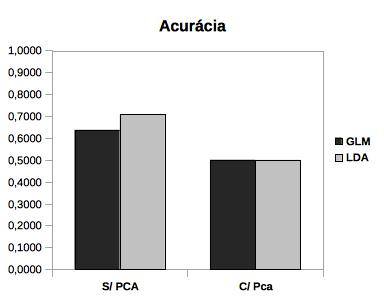
\includegraphics[scale=1.1]{acuracia}
  				\captionof{figure}{Gráfico das acurácias dos classificadores.}
			\end{center}
	     \end{solution}
		
		\pagebreak
		\paragraph{Anexo I: Código Fonte} 
		\lstinputlisting[language=R]{solutions.R}

		\end{questions}
		
\end{document}
